\documentclass{beamer}

\usepackage{ctex}
\usepackage{float}
\usepackage{xcolor}
\usepackage{pdfpages}
\usepackage{graphicx}
\usepackage{hyperref}
\usepackage[T1]{fontenc}
\usepackage{amsmath, amssymb}

\usepackage{UCAS}

\author{赵XX \quad 李XX \quad 蔡XX \quad Illusionna \quad 张旭橙博士指导}
\title{视觉问答中人与机器的认知分布差异分析}
\subtitle{智能人机交互开题报告}
\institute{第十组}
\date{\today}


\definecolor{deepred}{rgb}{0.6,0,0}


\begin{document}\kaishu



\begin{frame}
    \titlepage
    \vspace*{-1em}
    \begin{figure}[H]
        \begin{center}
            
\includegraphics[scale=0.2]{./figs/CAS_Logo.png}
        \end{center}
    \end{figure}
\end{frame}

\begin{frame}
    \tableofcontents[
        sectionstyle = show,
        subsectionstyle = show/shaded/hide,
        subsubsectionstyle = show/shaded/hide
    ]
\end{frame}



\section{选题动机与研究重要性}
\subsection{多模态理解任务的重要性}

\begin{frame}{2021 年 VQA 挑战赛}
    \begin{figure}[H]
        \centering
        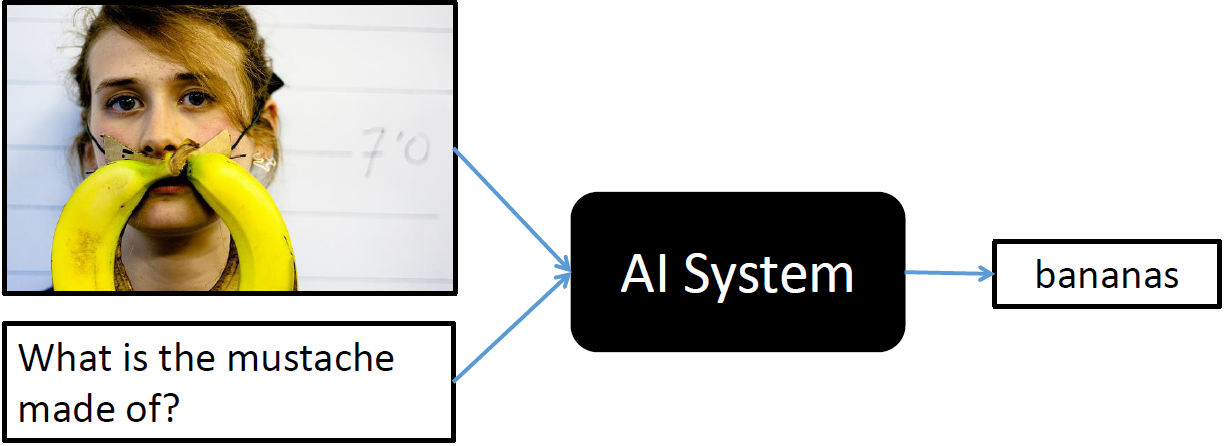
\includegraphics[scale=0.3]{./figs/challenge.png}
        \caption{\href{https://visualqa.org/challenge.html}{https://visualqa.org/challenge.html}}
    \end{figure}
    赛题描述：给定一张图片和一个关于该图片的自然语言问题，任务是提供准确的自然语言答案。
\end{frame}

\begin{frame}{多模态理解任务实际应用}
    \vspace*{-1.5em}

    \begin{columns}[T]
        \begin{column}{0.45\textwidth}
            \begin{figure}[H]
                \centering
                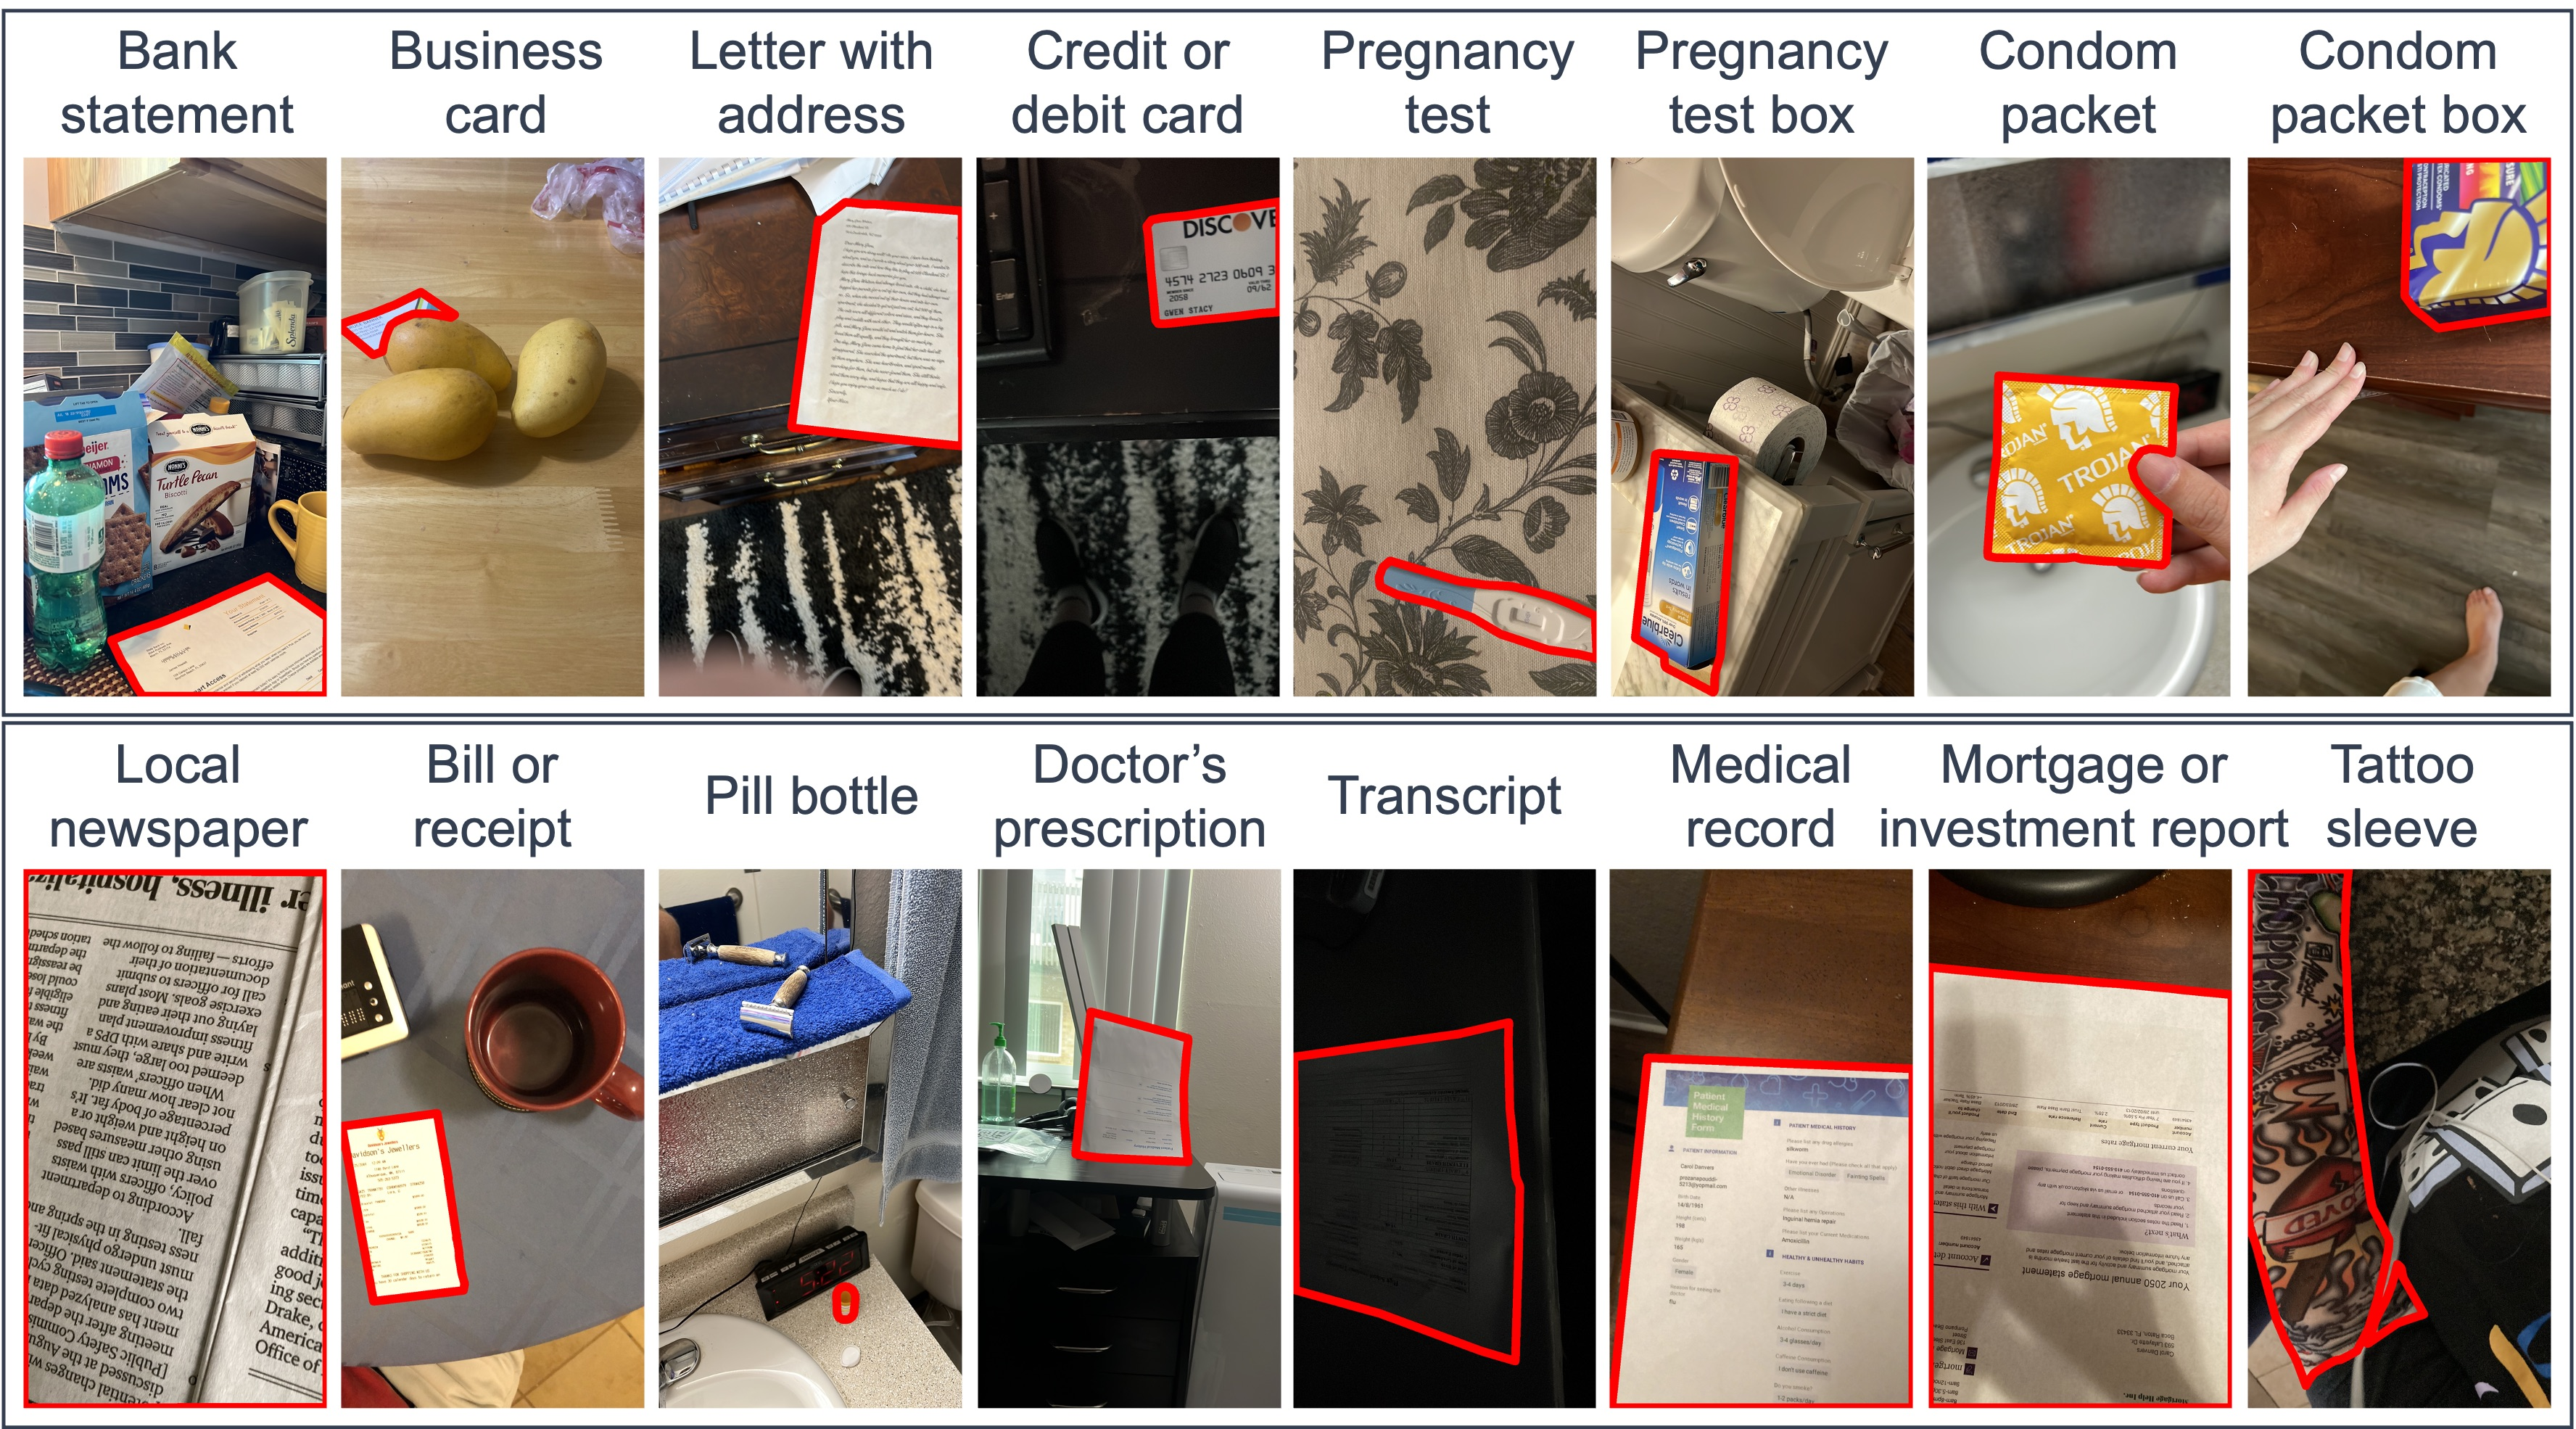
\includegraphics[width=\linewidth]{./figs/blind.jpeg}
                \caption{辅助盲人理解图像}
            \end{figure}
            \vspace*{-1em}
            \begin{figure}[H]
                \centering
                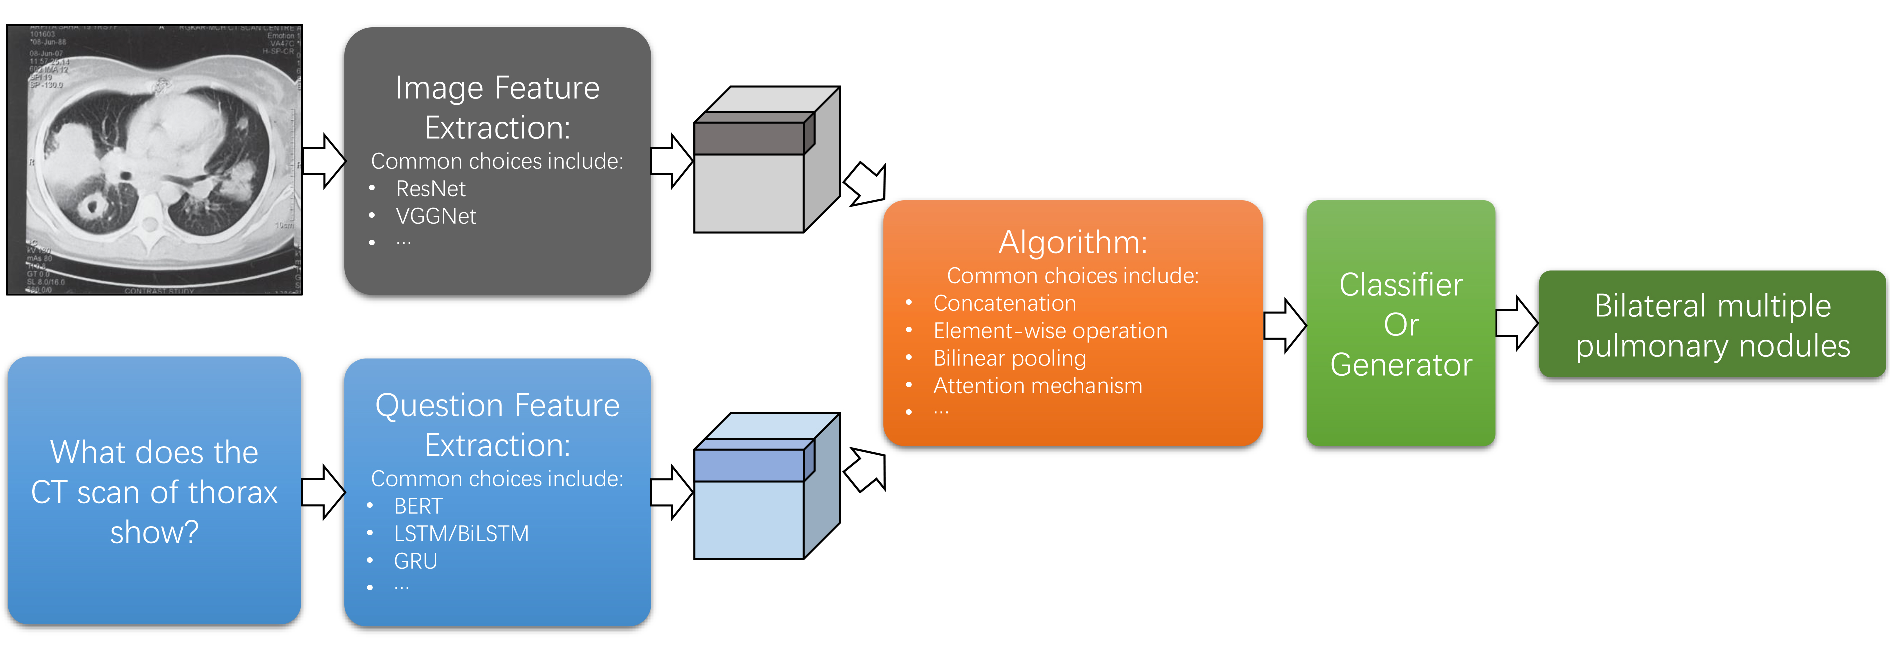
\includegraphics[width=\linewidth]{./figs/brain.pdf}
                \caption{医疗影像问答系统}
            \end{figure}
        \end{column}

        \begin{column}{0.45\textwidth}
            \begin{figure}[H]
                \centering
                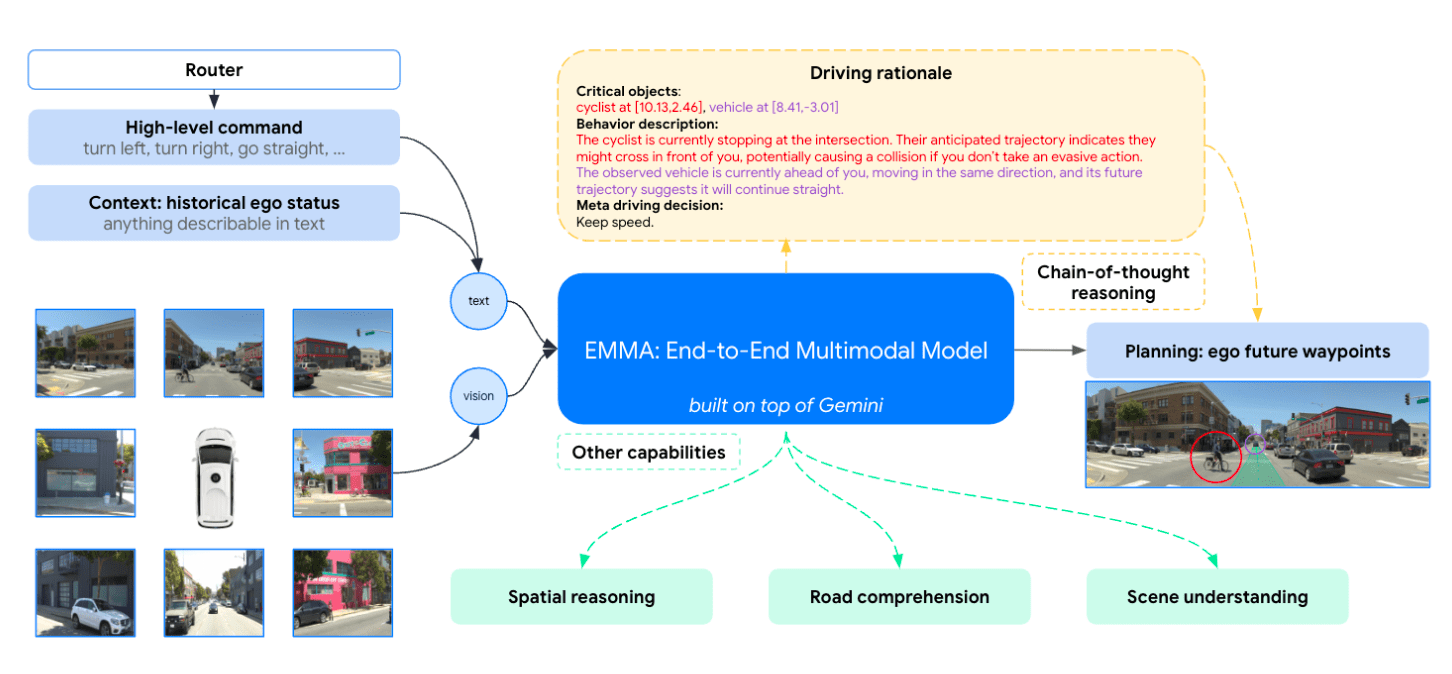
\includegraphics[width=\linewidth]{./figs/driving.png}
                \caption{自动驾驶场景理解}
            \end{figure}
            \vspace*{-1em}
            \begin{figure}[H]
                \centering
                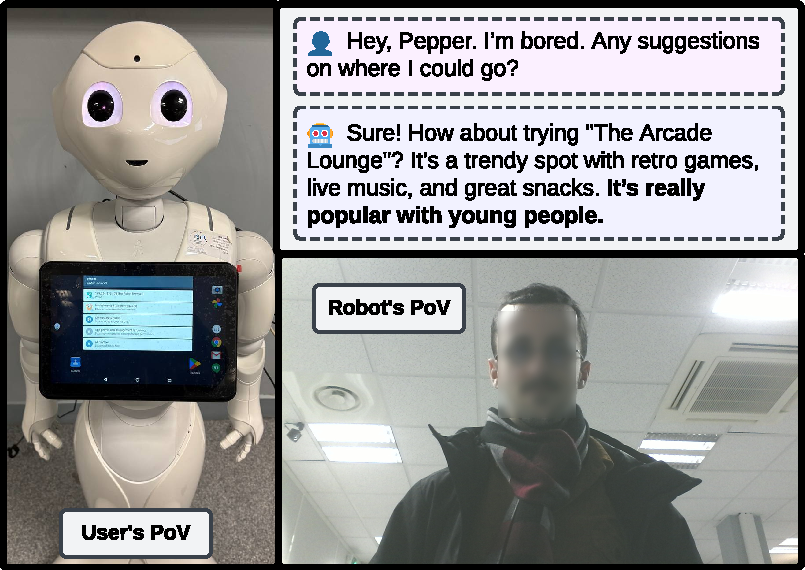
\includegraphics[width=0.65\linewidth]{./figs/robot.pdf}
                \caption{机器人与人的互动}
            \end{figure}
        \end{column}
    \end{columns}
\end{frame}



\subsection{注意力机制在 VQA 中的核心地位}

\begin{frame}{VQA 核心关注问题}
    \begin{figure}[H]
        \centering
        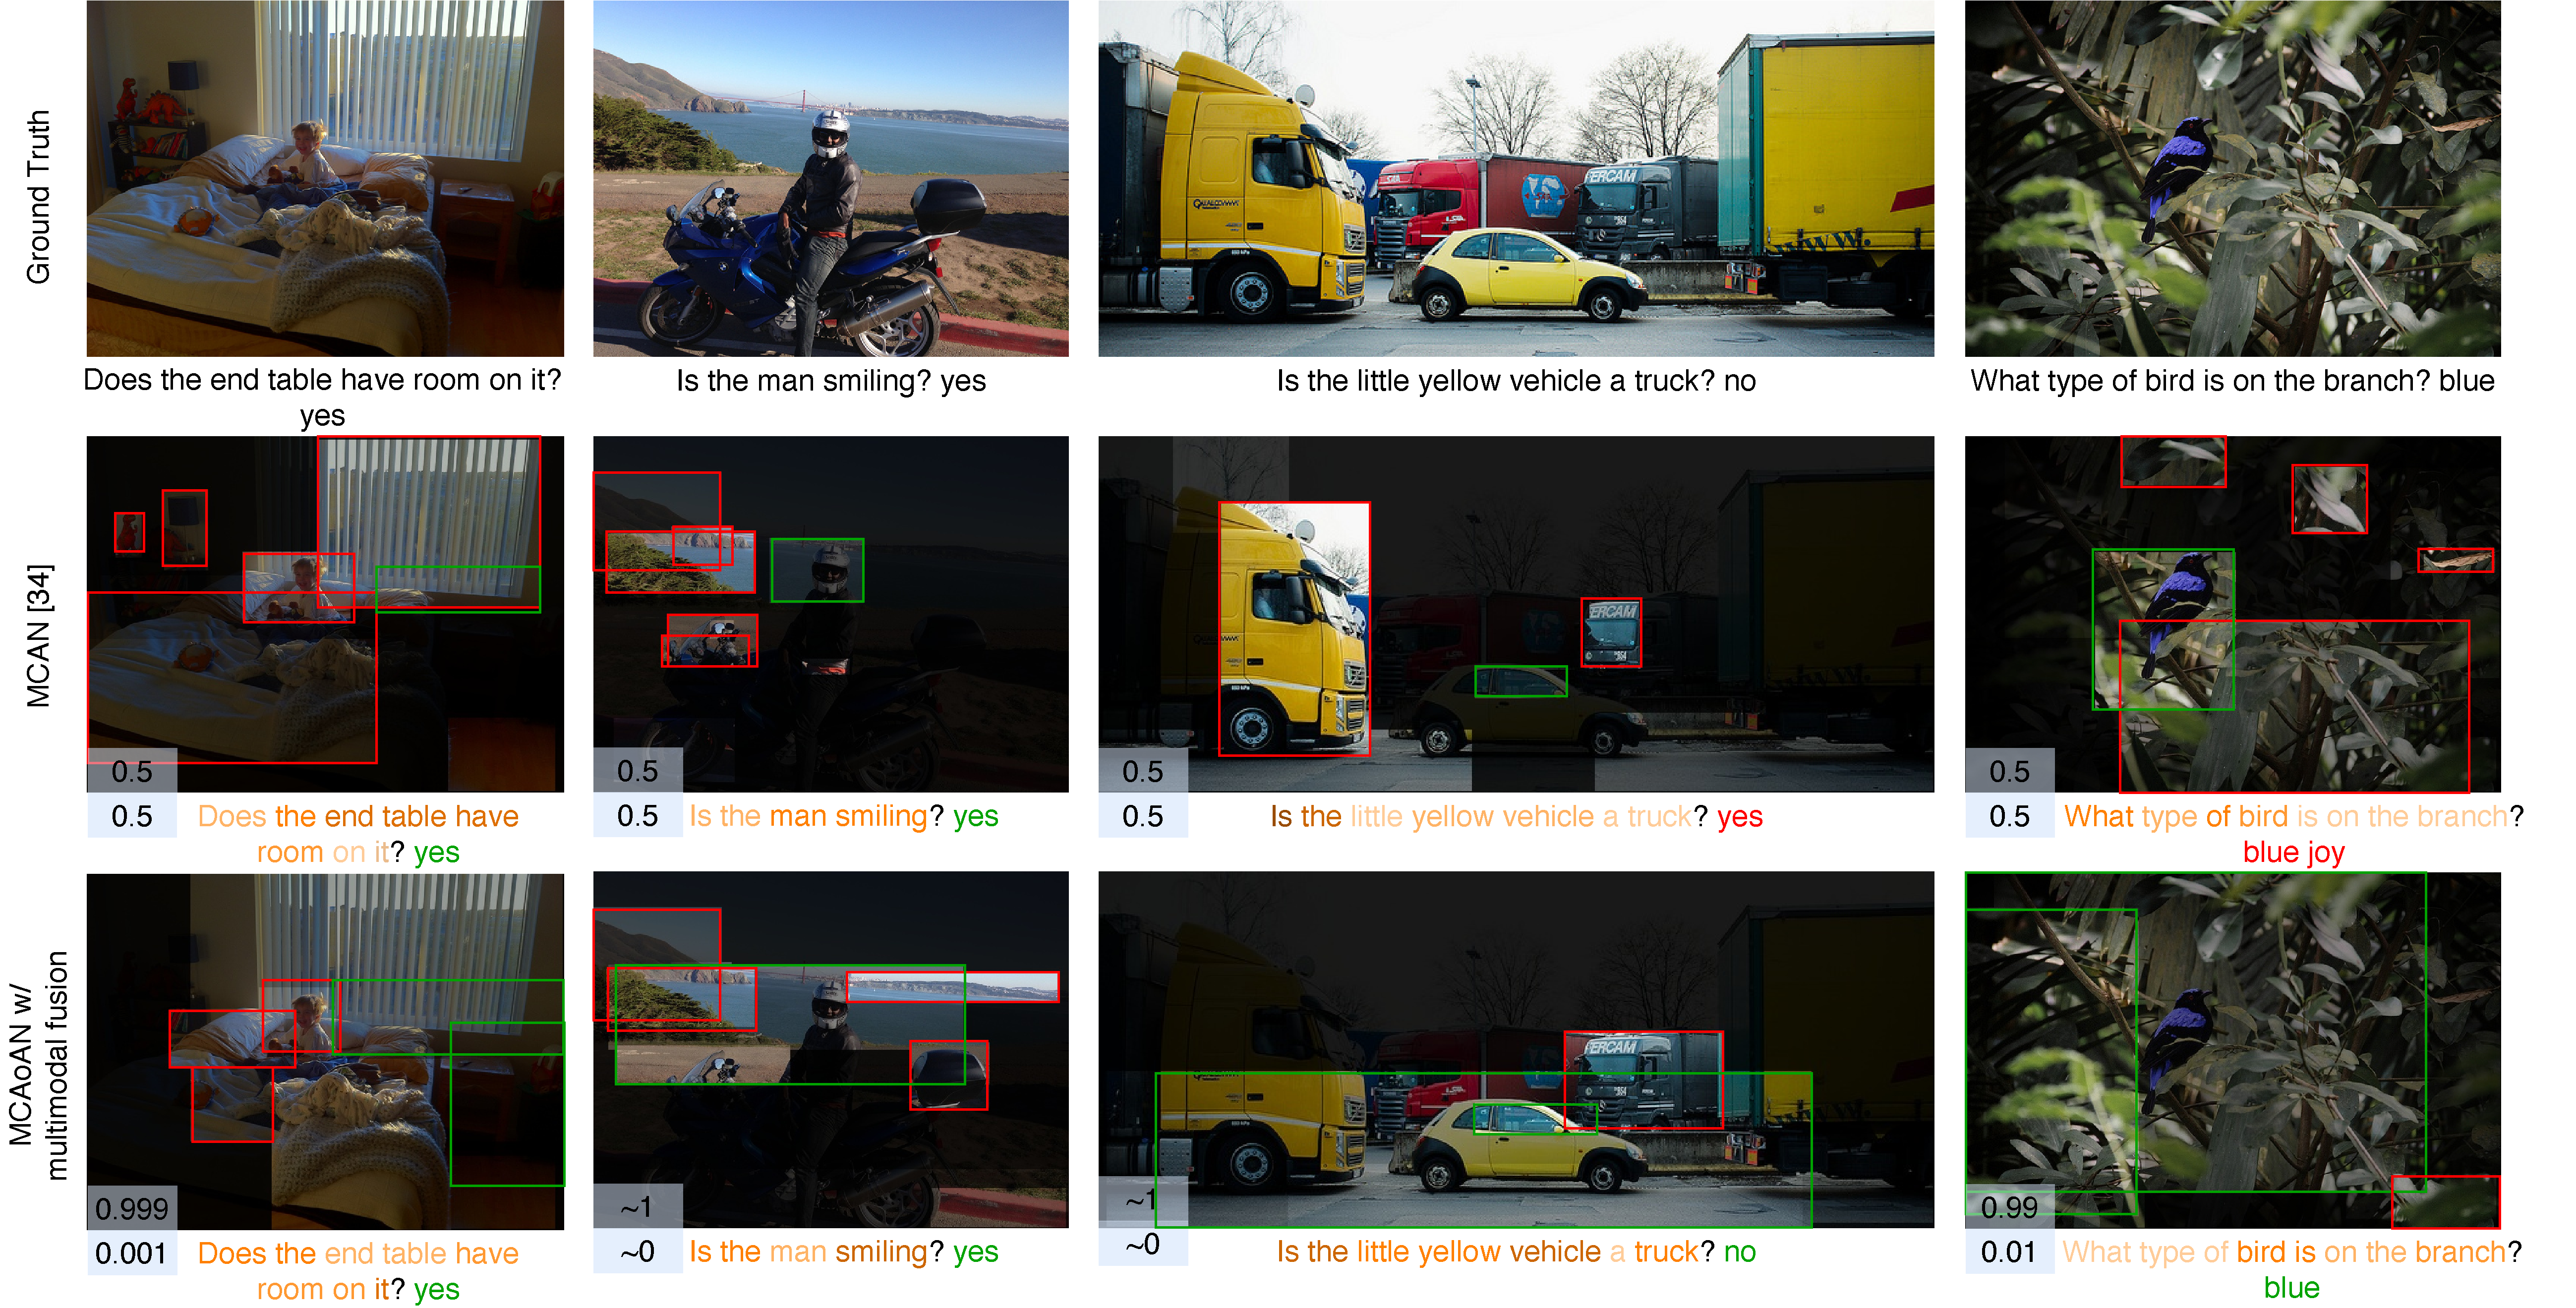
\includegraphics[scale=0.1]{./figs/qualitative.pdf}
        \vspace*{-0.5em}
        \caption{An Improved Attention for Visual Question Answering}
    \end{figure}
    \vspace*{-1em}
    VQA 关键问题：模型应该关注图像中的哪些区域？关注问题中哪些词语？即所谓的\textcolor{deepred}{\textbf{模型注意力分配问题}}。
\end{frame}

\begin{frame}{利用视觉语言注意力提升 VQA 模型性能}
    \begin{columns}[T]
        \begin{column}{0.48\textwidth}
            \begin{figure}[H]
                \centering
                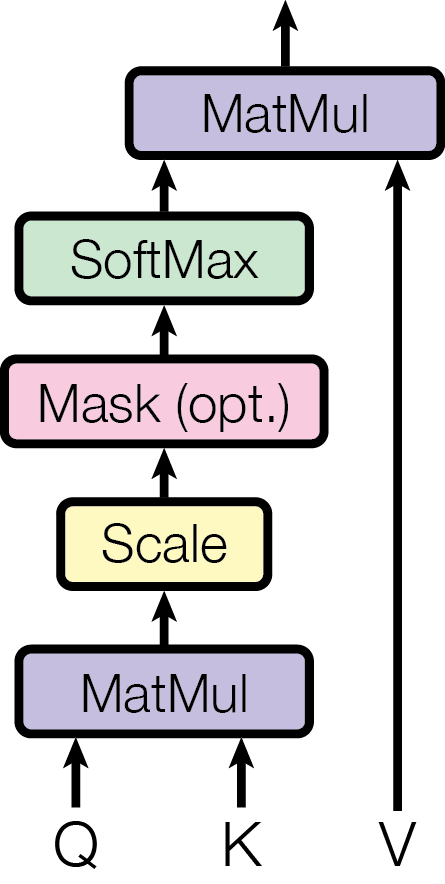
\includegraphics[width=0.5\linewidth]{./figs/attention.png}
                \caption{注意力机制}
            \end{figure}
        \end{column}

        \begin{column}{0.48\textwidth}
            \vspace*{3em}
            \textcolor{deepred}{\textbf{自注意力机制}}：通过计算输入元素（如图像区域或问题中的词）之间的相关性，生成加权的平均表示。这使得模型能够捕捉到图像中不同区域或问题中不同词语之间的关系，增强了模型的内部理解。
        \end{column}
    \end{columns}
\end{frame}

\begin{frame}{利用视觉语言注意力提升 VQA 模型性能}
    \begin{itemize}
        \item \textcolor{deepred}{\textbf{交叉注意力机制}}：通过利用两个不同模态（图像和问题）的特征，指导其中一个模态的信息流动。例如，词可以引导图像中的区域关注，从而建立两者之间的更紧密的关系。这种机制解决了传统注意力方法在图像和语言之间缺乏交互的问题。
        \item \textcolor{deepred}{\textbf{共注意力机制}}：将自注意力与交叉注意力结合，能够同时对图像和文本进行关注，从而加强它们之间的交互。它能使模型在推理时更好地对齐视觉和语言特征，提高理解能力。
    \end{itemize}
\end{frame}

\begin{frame}{VQA 注意力机制研究发展}
    \vspace*{-1.5em}
    \begin{figure}[H]
        \centering
        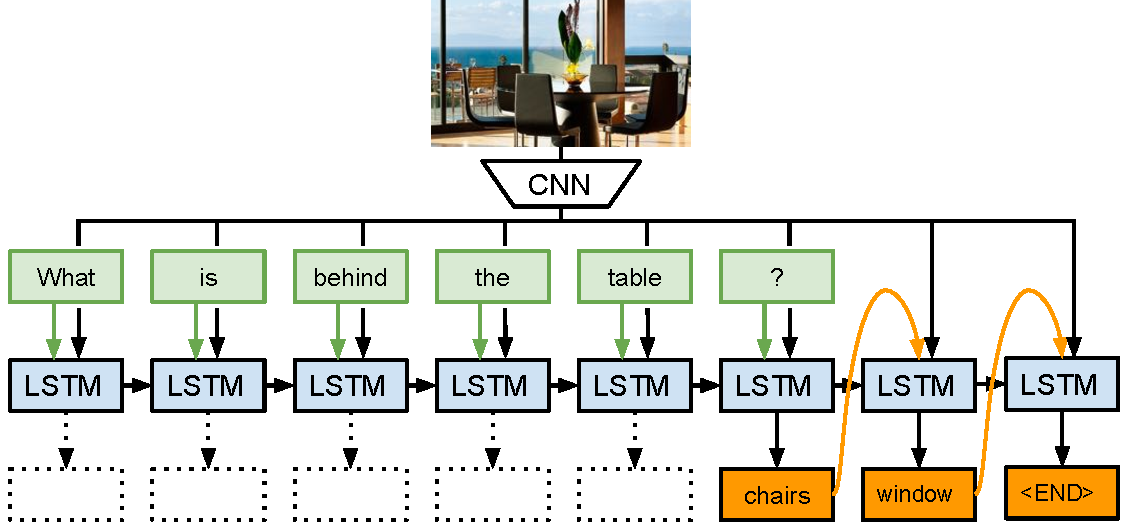
\includegraphics[width=0.75\linewidth]{./figs/QA-lstm.pdf}
        \caption{Ask Your Neurons: A Deep Learning Approach to Visual Question Answering}
    \end{figure}
    \vspace*{-1em}
    早期 VQA 多采用 CNN + RNN 的\textcolor{deepred}{\textbf{简单特征融合}}，无法区分图像与问题中的关键区域，视觉信息冗余、问题语义细粒度差异，使得模型需要一种机制来聚焦重要模态内容。
\end{frame}



\begin{frame}{VQA 注意力机制研究发展}
    当前 VQA 的注意力机制研究正成为热点：
    \begin{itemize}
        \item 空间注意力：聚焦图像中的关键区域，在“物体位置”“局部属性”类问题上表现突出，但缺少全局语义；
        \item 通道注意力：按特征通道分配权重，强调语义层面特征、类别相关性，但缺少空间分辨力；
        \item \textcolor{deepred}{\textbf{混合注意力}}：同时处理“哪里看”和“看什么”，提升多模态交互质量，更强的特征筛选；
        \item \textcolor{deepred}{\textbf{协同注意力}}：对图像特征和文本特征同时建模注意力，增强跨模特图文理解和动态双向依赖；
        \item \textcolor{deepred}{\textbf{重注意力}}：针对复杂问题进行多阶段反复关注，多步推理、逻辑链更长、表现更优。
    \end{itemize}
\end{frame}



\subsection{人类注意力分布 vs. 模型注意力机制}

\begin{frame}{人类与模型的关注存在差异}
    \vspace*{-1.5em}
    \begin{figure}[H]
        \centering
        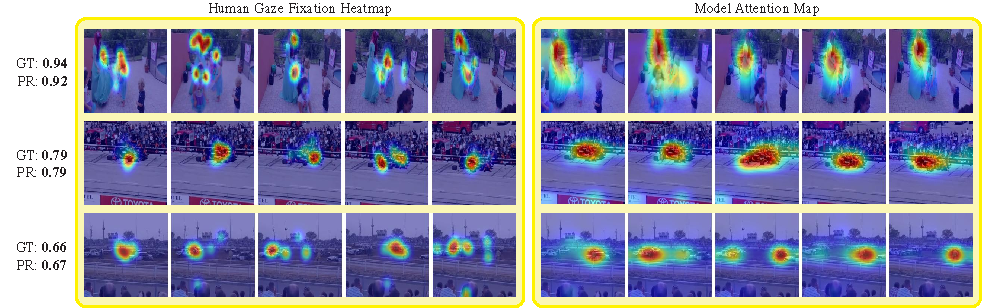
\includegraphics[width=\linewidth]{./figs/teaser_3rows.pdf}
        \caption{Seeing Eye to AI: Comparing Human Gaze and Model Attention in Video Memorability}
    \end{figure}
    \vspace*{-1.5em}
    \begin{itemize}
        \item VQA 模型生成的注意力往往与人类回答同样问题所关注的图像区域\textcolor{deepred}{\textbf{存在差异}}；
        \item 注意力的通用机制虽多，但多模态任务中“尚未完全解\textcolor{deepred}{\textbf{决跨模态对齐}}、\textcolor{deepred}{\textbf{细粒度注意力匹配}}、\textcolor{deepred}{\textbf{人类注意模拟}}”等问题。
    \end{itemize}
\end{frame}



\begin{frame}{人类与模型的关注存在差异}
    当前研究仍缺乏关键理解与突破：
    \begin{enumerate}
        \item 模型注意力机制\textcolor{deepred}{\textbf{为什么}}与人类注意分布存在差距？（例如是否侧重统计特征、语言提示、中心偏差、语言偏差）；
        \item \textcolor{deepred}{\textbf{如何设计}}注意力机制，使得模型等注意力分布更贴近人类注意方式，从而提升理解能力，减少错误关注区域性能；
        \item 注意力机制与推理过程，不仅是“看哪里”而且是“怎么看”以及“为什么看”，深入研究\textcolor{deepred}{\textbf{彼此之间的联系}}。
    \end{enumerate}
\end{frame}


\subsection{人机交互在 VQA 中的独特价值}

\begin{frame}{帮助机器学习到更符合人类认知模式的注意力分配}
    人类在解答视觉问题时，通常会选择性地聚焦于图像中的关键信息。人机交互能够通过获取人类的注意力反馈，让机器更好地模仿这种认知过程。与单纯依赖无监督学习不同，通过直接的交互，机器可以获取针对特定任务或问题的精准注意力指导，从而优化其注意力机制。例如，人类在回答“物体数量”问题时，通常会关注物体本身，而忽视背景细节。通过人机交互，机器能学习到这种动态选择性的注意力分配。
\end{frame}

\begin{frame}{有效缩小机器和人类之间在处理视觉任务时的差异}
    尽管深度学习模型在 VQA 任务中取得了不错的成绩，但现有模型的注意力机制通常无法与人类在任务中的表现对齐。人类注意力分布往往是灵活的、任务驱动的，而机器的注意力机制则多依赖于训练数据的统计特性。通过人机交互，可以直接从人类获取任务级别的反馈，帮助机器调整其注意力机制，使其更加符合人类的视觉认知方式。这样的交互使得机器能够理解哪些区域对特定任务至关重要，从而弥补当前模型在注意力分配上的不足。
\end{frame}

\begin{frame}{为机器提供强有力的监督}
    \vspace*{-1.5em}
    \begin{figure}[H]
        \centering
        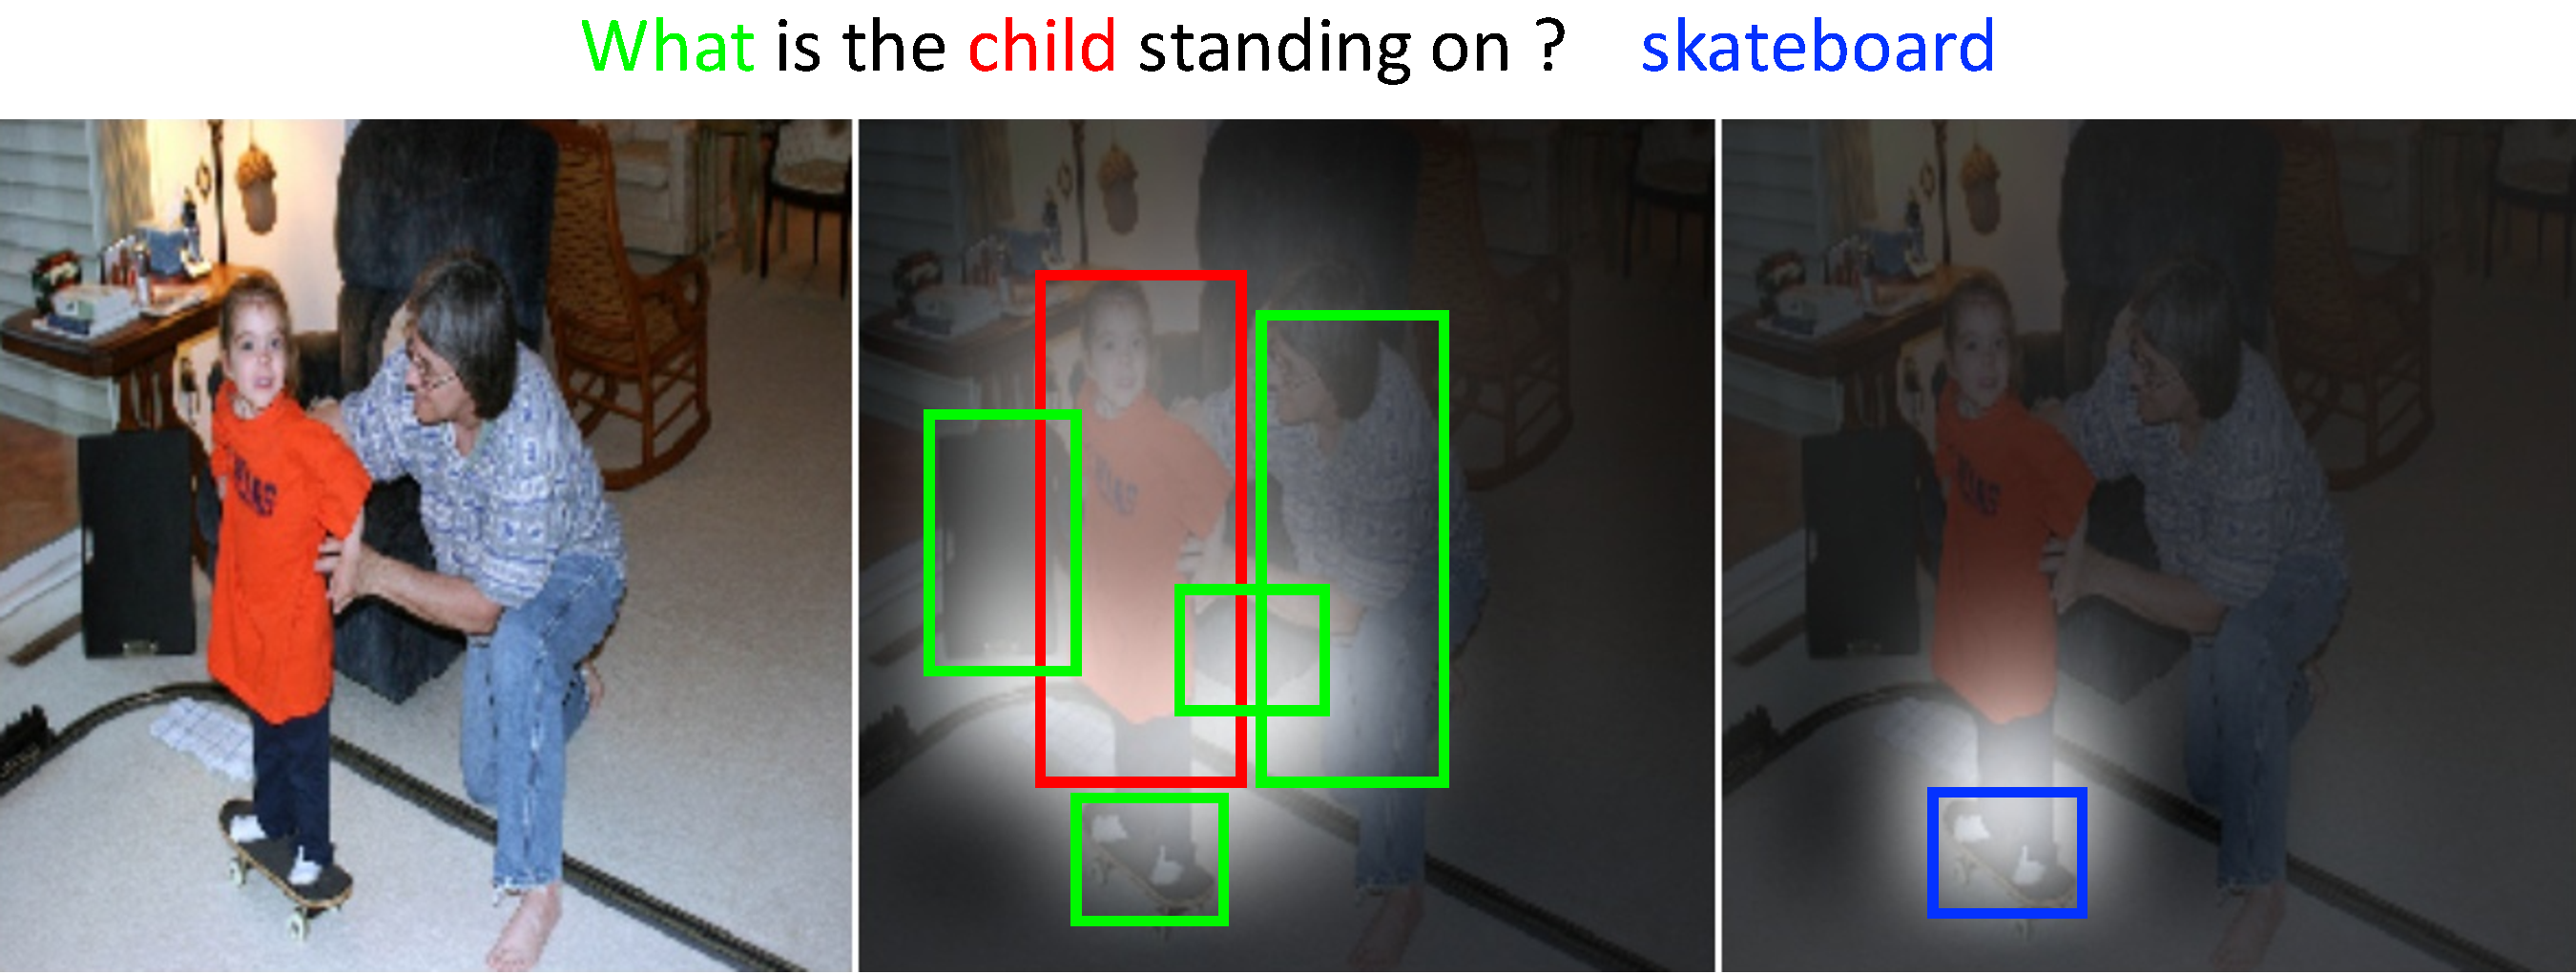
\includegraphics[scale=0.15]{./figs/concept_graph.pdf}
        \vspace*{-0.5em}
        \caption{Ask, Attend and Answer: Exploring Question-Guided Spatial Attention for Visual Question Answering}
    \end{figure}
    \vspace*{-1.5em}
    视觉任务的复杂性往往源于背景噪声、模糊的信息和多样化的物体。简单的深度学习模型在这些环境下往往失去精确度，因为它们难以有效过滤掉无关信息或聚焦于关键区域。人机交互提供了针对特定问题的反馈，能够帮助模型在训练过程中逐步修正其注意力焦点。例如，当背景信息过于复杂时，人类能够指出哪些区域与任务相关，哪些是噪声。这样的监督能够显著提高模型在处理复杂任务时的表现。
\end{frame}

\begin{frame}{提升 VQA 模型的可解释性}
    \vspace*{-1.5em}
    \begin{figure}[H]
        \centering
        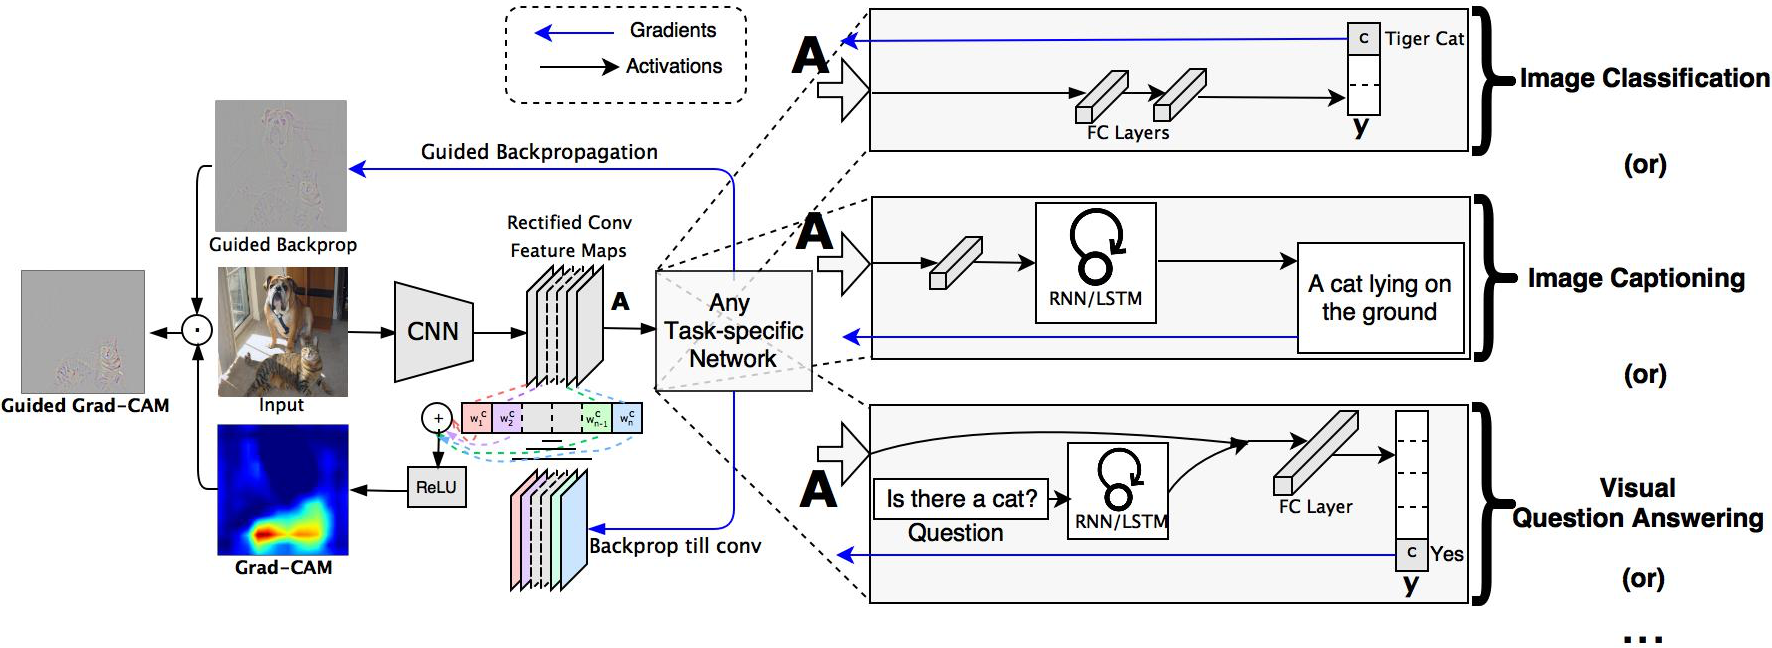
\includegraphics[scale=0.1]{./figs/Grad-CAM_approach.png}
        \vspace*{-0.5em}
        \caption{Grad-CAM: Visual Explanations from Deep Networks via Gradient-based Localization}
    \end{figure}
    \vspace*{-1em}
    当前的 VQA 模型往往在回答时提供高准确率，但其内部决策过程不易被理解。通过引入人机交互，机器不仅能学习到哪些图像区域与问题相关，还能使这一过程变得更加透明。用户可以通过可视化的注意力图看到模型为何做出某一答案，是否合理。这种透明度对于提升模型的可解释性至关重要，尤其是在涉及到高风险领域（如医疗影像诊断或自动驾驶）时，人机交互式训练能够使模型的决策过程更符合人类的逻辑推理。
\end{frame}



\section{相关研究综述}
\subsection{现有研究的进展}

\begin{frame}{注意力的 VQA 模型}
    \vspace*{-1.5em}
    \begin{figure}[H]
        \centering
        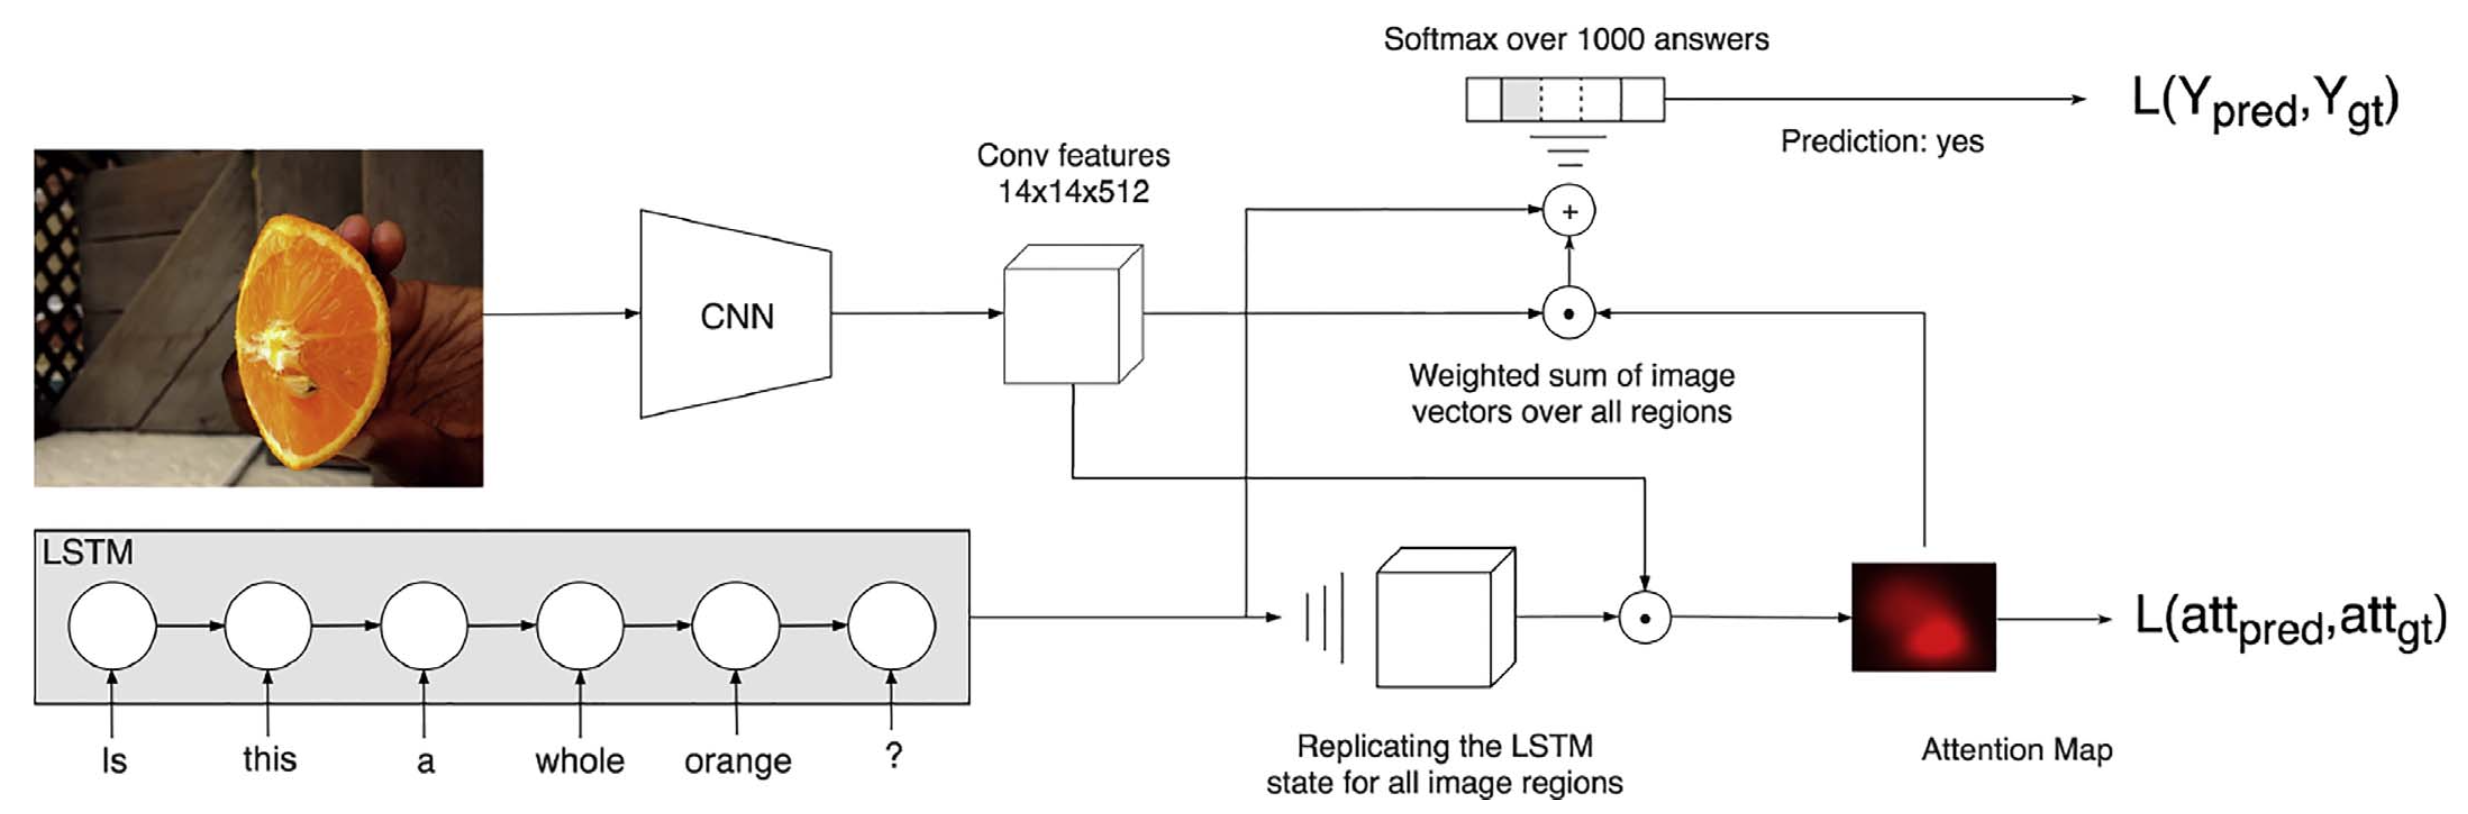
\includegraphics[scale=0.24]{./figs/SAN.png}
        \caption{Human Attention in Visual Question Answering: Do Humans and Deep Networks Look at the Same Regions?}
        \label{SAN}
    \end{figure}
    \vspace*{-1em}
    图~\ref{SAN} 是 SAN 堆叠注意力网络以及 HieCoAtt 分层协调注意力网络等，这些模型在图像文本配对回答问题时具有一定效果，通过\textcolor{deepred}{\textbf{在图像文本配对中引入注意力机制}}，强调图像中某些关键区域，借此提高对问题的回答能力。
\end{frame}

\begin{frame}{注意力的相关性评估}
    一些研究开始探讨人类和模型注意力分布之间的关系：
    \begin{enumerate}
        \item 虽然 SAN-2 和 HieCoAtt 等模型在能够识别与人类注意力相关的图像区域，但\textcolor{deepred}{\textbf{模型与人类实际关注的区域之间的相关性依然较低}}；
        \item 此类模型的注意力机制更多依赖于图像特征和语言描述之间的复杂交互，但\textcolor{deepred}{\textbf{忽视人类在解答图像问题的注意分布规律}}。
    \end{enumerate}
\end{frame}



\subsection{现有研究的不足}

\begin{frame}{现有研究的不足}
    \vspace*{-0.5em}
    \begin{itemize}
        \item \textcolor{deepred}{\textbf{注意力机制未完全模拟人类注意力}}：目前的 VQA 模型，在视觉问题的回答过程中，虽然通过注意力机制突出图像中的关键信息区域，但这些\textcolor{deepred}{\textbf{模型的注意力分布与人类的注意力区域并不一致}}，尽管模型可以预测出正确的答案，但其\textcolor{deepred}{\textbf{关注的图像区域常常偏离人类的视觉关注区域}}；
        \item \textcolor{deepred}{\textbf{“中心偏差”问题}}：模型倾向于集中关注图像中心的区域，这与人类的视觉习惯不符，当模型生成的注意力依赖于任务无关的显著性预测时，其中心偏差往往导致性能下降，为更好模拟人类视觉注意力，通过去\textcolor{deepred}{\textbf{中心化的注意力设计}}，提升模型的有效性；
        \item \textcolor{deepred}{\textbf{缺乏显式的注意力监督}}：当前注意力机制多通过无监督的方式进行训练的，缺少足够的显式监督来引导模型更加贴近人类注意力的模式，通过直接\textcolor{deepred}{\textbf{引入人类注意进行监督训练}}，能够有效提高模型在视觉问题中回答的准确性。
    \end{itemize}
\end{frame}



\section{研究内容与具体步骤}
\subsection{人类注意力分布采集与分析}

\begin{frame}{研究内容}
    \begin{itemize}
        \item 构建一套包含图像和问题的 VQA 数据子集，如 VQA-v2、GQA 等，\textcolor{deepred}{\textbf{在此子集采集或利用已有的人类注意力注释}}（例如手眼注视、鼠标追踪、高亮标注）；
        \item \textcolor{deepred}{\textbf{对人类在不同类型问题}}（例如数目类、位置类、属性类、推理类）\textcolor{deepred}{\textbf{下的注意力分布进行统计分析}}：关注区域在图像中的分布、与问题关键词的关系、与答案类型的关系；
        \item 分析人类注意力分布的规律性：例如人类是否\textcolor{deepred}{\textbf{优先关注}}目标物体、背景物体、语言提示区域，是否\textcolor{deepred}{\textbf{随着问题类型的变化而明显改变关注}}模式。
    \end{itemize}
\end{frame}


\begin{frame}{具体步骤}
    \begin{enumerate}
        \item 确定数据集与问题类型分类，如数目类、位置类、推理类等；
        \item 收集人类注意力数据，若已有数据（如 VQA-HAT）可使用，否则设计标注任务（例如鼠标点击、滑动高亮区域）；
        \item 对图像和问题生成注意力热图，并将人类多标注结果聚合为“人类注意力分布”；
        \item 使用统计方法（例如热图集中度、覆盖率、与物体边界重叠度）对不同类别问题下的人类注意力进行比较分析；
        \item 总结人类关注行为的特点、规律、差异（例如哪些类别问题人类多关注背景、哪些类别关注目标物体）。
    \end{enumerate}
\end{frame}



\subsection{现有 VQA 模型注意力机制评估与对比分析}

\begin{frame}{研究内容}
    \begin{itemize}
        \item 选取几个具有\textcolor{deepred}{\textbf{代表性的 VQA 模型}}（例如含有注意力机制的模型、共注意力模型、Transformer-based 模型）在相同的图像和问题配对中提取模型的注意力；
        \item \textcolor{deepred}{\textbf{对比模型产生的注意力分布与人类注意力分布}}，包括区域重叠率、关注中心距离、关注词语与物体匹配度、是否存在“错误关注”区域，譬如模型将注意力分配到与问题无关背景；
        \item \textcolor{deepred}{\textbf{分析模型注意力机制中存在的不足}}，例如模型侧重中心区域、过度依赖语言提示、忽略关键细节、关注区域模糊或分散、对背景干扰敏感等。
    \end{itemize}
\end{frame}

\begin{frame}{具体步骤}
    \begin{itemize}
        \item 选定模型，譬如 MCAN、Dense Symmetric Co-Attention；
        \item 提取注意力权重图像区域关注概率；
        \item 量化模型注意力图与人类注意力图的差距，可采用指标如 IoU 重叠度、KL 散度（分布差异）、关注中心偏移距离等；
        \item 对比不同问题类型下模型和人类注意力差异情况，找出“差异大的问题类型”、模型容易犯错的区域分配模式、关注机制可能的缺陷；
        \item 总结分析，指出现有模型在注意力机制上“已经做到”的程度，例如对目标物体的关注、与语言提示的融合，“还未做到”的问题，例如对背景细微语境的关注、跨模态推理注意力的有效分配等。
    \end{itemize}
\end{frame}



\subsection{设计改进的注意力机制}

\begin{frame}{研究内容}
    \begin{itemize}
        \item 基于分析结果，提出一种改进方案，例如\textcolor{deepred}{\textbf{引入人类注意力监督、去中心偏差模块、背景干扰抑制机制、跨模态推理注意力模块}}；
        \item 设计相应的模块架构，将其整合到现有的 VQA 模型中，\textcolor{deepred}{\textbf{作为插件模块}}；
        \item 在人类注意力的基础上，生成注意力先验，用于\textcolor{deepred}{\textbf{监督模型训练}}，加入对问题类型\textcolor{deepred}{\textbf{自适应的注意力分配机制}}，引入\textcolor{deepred}{\textbf{多步注意力演化机制}}，模拟人类先看整体，再关注细节。
    \end{itemize}
\end{frame}


\begin{frame}{具体步骤}
    \begin{itemize}
        \item 分析得到规律，人类回答“数目类”问题时更多关注目标物体集群，而模型却关注中心背景；
        \item 针对这些具体规律，设计模块或机制：
        \begin{itemize}
            \item 注意力先验模块：将人类关注作为\textcolor{deepred}{\textbf{额外损失监督}}模型注意力分布；
            \item 注意力修正模块：\textcolor{deepred}{\textbf{对模型注意力进行纠偏}}，如抑制背景区域、增加目标区域权重；
            \item 多步注意力演化：\textcolor{deepred}{\textbf{模型分多步生成注意力}}，从粗到细，模拟人类“整体”到“细节”关注流程；
        \end{itemize}
        \item 将改进模块集成到基础 VQA 模型中，调整训练流程，例如引入联合损失，回答损失与注意力分布损失；
        \item 实现并训练模型，在相同数据集上与基线模型进行对比。
    \end{itemize}
\end{frame}



\subsection{实验验证、分析}

\begin{frame}{研究内容}
    \begin{itemize}
        \item 在相同数据集问题类型上对改进模型进行实验，比较其与基线模型在人类关注匹配度、回答准确性、可解释性等维度上的提升；
        \item 深入分析不同问题类型改进效果的差异、注意力分布变化情况、可能的失败案例及其原因总结研究贡献、提出未来工作方向。
    \end{itemize}
\end{frame}

\begin{frame}{具体步骤}
    \begin{itemize}
        \item 准备实验环境、数据集训练基线模型与改进模型；
        \item 整体和按照问题类别的 VQA 回答准确率，模型注意力热图与人类注意力的匹配度指标，例如 IoU、KL 散度、中心偏移；
        \item 可解释性分析，可视化模型注意力图，定性分析其关注区域是否合理；
        \item 对比分析改进模型与基线模型在上述指标上的差异，并分析哪类问题改进最多、哪类问题仍有缺陷；
        \item 撰写结果报告，指出，是否达到了预期“模型注意力更贴近人类”，是否提升了 VQA 回答性能，模型在可解释性上是否有所增强，存在的局限，如难以处理极端背景、推理类问题仍旧差距较大；
        \item 提出未来工作建议，扩大人类注意力数据集、处理更多问题类型、进一步提升跨模态推理能力。
    \end{itemize}
\end{frame}



\section{预期成果}

\begin{frame}{预期成果}
    \begin{enumerate}
        \item 改进后的模型在 VQA 任务上能够取得显著优于基线模型的回答准确率，尤其是在那些\textcolor{deepred}{\textbf{人类注意力分布规律}}明显，但基线模型关注不佳的问题类型（如位置类、属性细节类、复杂背景类）；
        \item \textcolor{deepred}{\textbf{模型生成的注意力图与人类注意力图的匹配度提升}}（例如 IoU 增加、KL 散度减少、中心偏移减小）；
        \item \textcolor{deepred}{\textbf{模型的可解释性增强}}，通过可视化注意力图，用户能够更直观看到模型“为什么”选取某些区域、更贴近人类推理过程；
        \item 注意力机制需要结合\textcolor{deepred}{\textbf{人类关注模式、跨模态对齐、背景干扰抑制、问题类型自适应等机制}}才能更好地提升 VQA 模型。
    \end{enumerate}    
\end{frame}


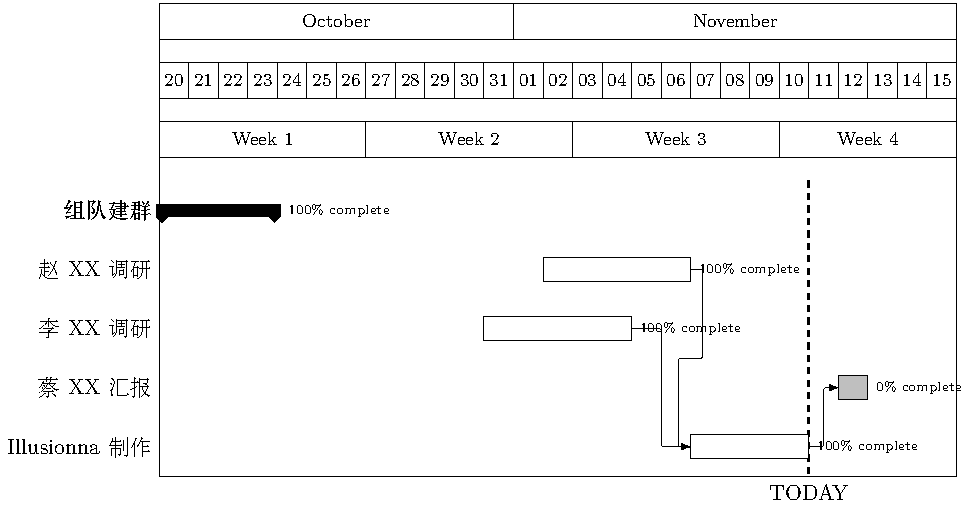
\includepdf[pages=-]{./documents/progress.pdf}


\end{document}